\documentclass{report} 
\usepackage[utf8]{inputenc}
\usepackage{graphicx}
\usepackage[margin=1.5in]{geometry}
\usepackage{lingmacros}
\usepackage{verbatim}
\usepackage{subfig}
% exempel: 2) Inte vet jag
%              not know I
%             I don't know

\begin{document}
% ska gå att förstå och locka till läsning
%ska tydligt beskriva vad rapporten handlar om
%ska innehålla vettiga sökord
\title{Scaling up a GF grammar and preparing it for cool stuff for Swedish}
\author{Malin Ahlberg}
\maketitle
\newpage

\tableofcontents
\newpage

\abstract{
% This is the report of the work of expanding a GF grammar and preparing
% it for parsing of free Swedish. A lexicon consisting of more than 100 000 words
% has been extracted and we have constructed an automatic mapping between the
% annotation of the treebank Talbanken and GF. 
% The goal is to build a robust parser dealing with uncontrolled natural
% language, a parser which, for example, can parse all of Talbanken.
% Outside of this project, an equivalent GF project for English is being worked upon,
% as are theqniques for making the parser robust.
% With this in mind, we have extended the current GF grammar to adapt it for
% Swedish specifically so that it can parse the an extended set of basic
% constructions. We have completed a method for importing the eletronical 
% lexicon Saldo to a GF format and upprätat en connection mellan oss och Talbanken.

% sf dream to be able to work with npl. Parser important, statistics working
% on n-grams fail, closer to the human brain with rules? 
% Describe the basic.. of Swedish, in a format compatible with 20 other languages.
% example of sentence and how it can be parsed, stepping out of the controlled lang.
% Combine other resources, create free software.
% Equivalent for English and other languages coming.
% We aim for free parsing, this is preparation and up-scaling, finding difficulties.
}

\newpage

\section*{Acknowledgements}
% Ramona, Aarne, Elisabet, Markus, Peter?, Lars, Dan, Krasimir etc

\newpage
\chapter{Introduction}
\section{Introduction} 
Ultimate goal: want computers to 'understand' language. Not good with flat strings.
We need to translate strings of natural language to a richer sturture,
a parse tree. So far there is no
freely availbe ruled-based parsing giving a deep analyse for Swedish.
%There are parsers which put only put part-of-speach tags to
%the text, and others that gives a deeper analyse. 
There are statistical parser, and parser which only are deal with controlled language.
The GF parser are one of those. 
%What is parsing, flat strings to trees, example picture, what is deep parsing.
So far stable and good when working with controlled languges, but recent experiments
have showed that it is also possible to parse free language.
To do this for Swedish, we need to  .. the resource grammar needed to covering
the language specific constructions. Further a lagre lexicon is also needed, as well
as a method for evaluation.
During this project, we have worked on and explored those things and some problems identified.
We have extended the Swedish resource grammar in GF, to give a better coverage and imported
a large lexicon. Work to compare the trees from Talbanken to GF and to translate them.


%What is controlled language,
%what is robust parsing and why we need it for free langugae, benefits of a grammar.
%GF is grammar formalism, many languages, many projects for controlled lang.
%GF grammar for Swedish, how big, not intended for parsing, but for building
%application grammars. Experiments of using the grammar for free parsing, methods
%being developped for this. Benefits of starting from GF. Free parsing is
%interesting. To do this, we need a better (bigger grammar), a large scale
%lexicon, and an evaluation method. This project has explored those things. The
%grammar also have other usages, important in itself, so we wanted to make it as
%covering as possible without being overallowing or too ambiguous.

Other work exist, but none is freely available. We want to create a open source
product, therefore can only use resources that allows this. Work can continue,
will not disappear, be made use of in other projects.
What we could not cover by this project, what have been covered before (in
the spring project), and why we choose those parts.

\section{Background}  
To build a parser or a grammar from scratch is a heavy work. The idea for this
project is to combine already existing parts into a bigger and more expressive grammar
as well as a large scale GF lexicon.
As all GF grammars, this one can be used for parsing, and we develop it by getting
examples, ideas and test material from a treebank.
The project is hence heavily dependening on three resources, which will be described
in the following sections.

\subsection{Swedish}
Swedish\cite{SAG:intro} is a North-Germanic language,
closely related to Norweigan and Danish. The languages share most of their
grammatical structures and are mutual intelligibility. Swedish is also 
an official language in Finland and spoken by approximately 10 million people.
Swedish syntax are often similair to English, but have some characteristics:
\subsubsection*{Verb second}
Swedish is a verb-second language: the
second constituent of a declarative main clause must consist of a verb.
The normal word order is subject-verb-object, but any syntactic category can be fronted\cite{H&H:1027}.
Topicalisation is very common, especially for temporal and spatial adverbial phrases.
The examples \ref{ex:swedish-svo} - \ref{ex:swedish-avso} all have the same propositional
meaning, although the fronted part of sentence \ref{ex:swedish-ovs} and \ref{ex:swedish-avso} are being emphasized.
\enumsentence{
\shortex{4}
{Du & ser & mig & inte.}
{You & see & me & not.}
{`You  don't see me'.}} \label{ex:swedish-svo}
\vspace{-3mm}
\enumsentence{
\shortexnt{4}
{Mig  & ser &  du & inte.}
{Me & see & you & not.}}\label{ex:swedish-ovs} 
\vspace{-3mm}
\enumsentence{
\shortexnt{4}
{Inte & ser& du &mig.}
{Not&  see& you& me.}} \label{ex:swedish-avso}

%\shortexm{3}
%{hej} {hi}{hhe} {bing}{bong}{salt}
%; adverbials, objects
%Alla syntaktiska kategorier kan be fronted utom obetonade satsadverbial (ju,väl).
%The first constituent of the clause is usually made up of the subject,
%although it likewise could consist of adverbial phrases or objects that are
%being empathazied. \\
%\enumsentence{
%\begin{tabular}{lll}
%  Johan & gick & sakta på gatan.\\
%\emph{Johan} & \emph{walked} & \emph{slowely on the street.}\\
%  Sakta & gick & Johan på gatan.\\
%\emph{Slowly} & \emph{walked} & \emph{Johan on the street.}\\
%  På gatan & gick & Johan sakta.\\
%\emph{On the street} & \emph{walked}  & \emph{Johan slowly.}\\
%\end{tabular}}

Inverted word order marks questions
\enumsentence{
\shortex{4}
{Såg & du & mig & inte?}
{Saw  & you&  me& not?}
{`Didn't you see me?'}}
%\enumsentence{Gick Johan på gatan?\\
%        \emph{Did Johan walk on the street?}}
The word order in subordinate clauses in also slightly different,
%\enumsentence{
%\begin{tabular}{ll}
%{\shortex{7}
%{Jag & såg&  Anna.&  Hon & såg & inte&  mig.} 
%{ & & &  & & &}}
%\shortex{7}
%{Jag såg att Anna \textbf{inte} såg mig.}\\
%\shortex{7}
%{I  saw Anna. She saw not   me.}  & {I   saw that Anna not saw me}. \\
%`I saw Anna. $\;$ She did not see me.'& `I saw that Anna did not see me'.
%}
\enumsentence{Main sentences:\\
{\shortex{7}{Jag & såg & Anna. & Hon & såg & {\bf inte} & mig }
{ I & saw & Anna. & She & saw & {\bf not} & me}
{`I saw Anna. She didn't see me'}}}
\enumsentence{Subordinate sentence:\\
\shortex{7}{Jag & såg & att& Anna& \textbf{inte}& såg& mig.}
            {I &  saw & that& Anna& \textbf{not}& saw& me.}
            {`I saw that Anna didn't see me'}} 

\subsubsection*{Passive voice}
Passive voice is often used in Swedish, especially the
\textit{s-passive}, which is formed by adding an \emph{s} at the end of a verb.
\enumsentence{Passive \hspace{39mm} Active\\
\shortexm{11}{Han & jagade\textbf{s} & av & ett & lejon.}
        {He & hunted+\textbf{s} & by & a & lion.}
        {`He was hunted by a lion.'}
{Ett & lejon & jagade & honom.}
        {A &lion &hunted &him.}
        {`A lion was hunting him.'}}


%cf.
%\enumsentence{
%\shortex{5}{Ett & lejon & jagade & honom.}
%        {A &lion &hunted &him.}
%        {`A lion was hunting him.'}}

\subsubsection*{Impersonal constructions}
Constructions with 'det är/var' ('it is/was') is very common\cite{H&H309d}:
\enumsentence{
\shortex{6}{Det & var & roligt & att & höra.}
{It &was & nice &to &hear.}
{`I'm glad to hear that.'}}
'Det' (\emph{it}) is also used as formal subject %for intransitive verbs,
with the real subject put in the position of an object.
\enumsentence{
\shortex{6}{Det &står &en &älg &på &fältet.}
{ It & stands &a & moose &on &the field.}
{`There is a moose on the field.'}}

\subsubsection*{Reflexive pronouns}
The Scandinavian language have reflexive pronouns\cite{H&H310}
and special reflexive forms of the possessive pronouns for the 3rd
person\cite{H&H319}. Those are distinct from the normal 3rd person forms.
\enumsentence{
\begin{tabular}{ll}
Han slog \textbf{sig}. & Han såg \textbf{sitt} barn.\\
\vspace{3mm}
\emph{He hit him self.} & \emph{He saw his (own) child.}\\
Han slog \textbf{honom}. & Han såg \textbf{hans} barn.\\
\emph{He hit him (another person).}&\emph{He saw his (another person's) child.}
\end{tabular}}
The 1st and 2nd persons use the normal personal pronoun in object form.


Could varandra be thought of as reflexive for 'oss'?
%Basic info about Swedish. V2 lang, inverted word order and subordinate clauses.
%Passive, reflexive 'sitt', 'det är', 'det sitter en katt där', prepare the reader
%for what will be written in the grammar part.
%Adjectives but not verbs congruate with nouns. De är stora, They are big, Jag
%är stor, I am big
%Since the s-passive is the most common one in written Swedish \cite{SAG-34-1}, it has


\subsection{Saldo}
A good parser needs a good lexicon. We have used of Saldo\cite{saldo}, a
large electronic lexicon developed and maintained at Gothenburg University. It is
built upon Svenskt Associations Lexicon and contains information about modern
Swedish and the words are equipped with both sematic and a morphological
information. The user can find compounding analyses, examples of usage in corpora,
and graphs of sematically connected words.\\
Example of katt? \\
For our purpose however, only the morphological data was needed.\\
Example of morpho for katt.\\
Saldo provides this in XML format under LPGL. The data can be processed and
translated to GF format as described in 
section \ref{sec:prog.saldo}.
%Other usages?


\subsection{GF}
The main component of the the project is the Grammatical Framework\ref{gfbok} (GF). It is
a functional grammar formalism based on Martin-Löf type theory.
It has been developed for about 20? years and are inspired by programming langauges
like Haskell\footnote{}, ML\footnote{}, Prolog\footnote{} and Agda\footnote{}. Grammars written in GF can be used together with languages 
like Java, Java script and Haskell and works for both parsing and generation.

Being developed with multilinguality in mind, GF makes an important distiction between
\textit{abstract} and \textit{concrete} syntaxes. The abstract is meant to be
shared by many languages, it models the semantics of the domain without blanda in
language specific features such as agreement or word order.

\begin{figure}[h]
\begin{verbatim}
 abstract TestGrammar = {
  cat N ; V ; S ;

  fun 
    Pred : N -> V -> S ;
    cat_N : N ;
    sleep_V : V ;
 }
\end{verbatim}
\caption{A small example of an abstract syntax}
\end{figure}

The example shows an abstract grammar defining three categories, % \verb|Categories|,
one for nouns, one for verbs and one for sentences. An abstract grammar also gives
the types of functions. In this case we have \verb|Pred| which
tells us that by taking a noun and a verb we can form a sentence. At this stage, 
no information of how this is done is given. The grammars also defines two words,
\verb|cat| and \verb|sleep|. 

% or how any of the categories should look.
\begin{figure}[h]
\begin{verbatim}
concrete TestGrammarSwe of TestGrammar = {
  lincat N, V, S = Str ;
   
  lin Pred n v   = n ++ v ;
      cat_N   = "katten"  ;
      sleep_V = "sover"  ;
}
\end{verbatim}
\caption{A Swedish concrete grammar}
\label{fig:gfSweCnc1}
\end{figure}

Figure \ref{fig:gfSweCnc1} shows how the abstract grammar can be implemented
for Swedish. Nouns, verbs and sentences are all defined as strings, \verb|Str|
and \verb|Pred| simply glues the two strings ``katten" and ``sover" together:
\verb|Pred cat sleep = "katten sover"|.\\
Let's look at a more complicated example, where nouns can be used in both
plural and singular. To do this, we add a category \verb|NP| to the
abstract. \verb|N| now means a noun
in any of the number, and we introduce two funciton, \verb|NSg : N -> NP| and
\verb|NPl : N -> Pl| which sets the number.
\begin{figure}[h!]
\begin{verbatim}              
 abstract TestGrammar = {          concrete TestGrammarSwe of TestGrammar = {
  cat N ; NP ; V ; S ;               lincat V, S, NP = Str ;
                                            N = {s : Num => Str} ;
  fun                                lin   
    Pred : NP -> V -> S ;              Pred n v = n ++ v ;
    NSg : N -> NP ;                    NPl n = n.s ! Pl ;
    NPl : N -> NP ;                    NSg n = n.s ! Sg ;
    cat_N : N ;                        cat_N = {s = table {Sg => "katten" ;
    sleep_V : V ;                                          Pl => "katterna"}};
 }                                     sleep_V = "sover"  ;
                                     param Num = Sg | Pl ;
                                     }
\end{verbatim}           
\caption{A modified grammar}
\label{fig:gfTest2}
\end{figure}
Figure \ref{fig:gfTest2} introduces some new concepts: records,tables and parameters.
In the concrete syntax, \verb|N| is defined to be a record consisting of the field
\verb|s|. The type of \verb|s| shows that it is a table, which given a parameter of type \verb|Num| returns
a string. \verb|Num| is defined as a parameter, which can either have value \verb|Sg|
or \verb|Pl|. In \verb|NPl| and \verb|NSg|, \verb|n.s| means that we use the
field \verb|s| of \verb|n|, and then the selection operator \verb|!| is used to
select a branch in the table.

If we want to implement a English version of the grammar, we encounter another
problem: the verb form depends on the noun phrase. The \verb|NP| needs to carry
information about which number it is in, and \verb|Pred| can pass this on to the
verb. Hence, the \verb|V| also needs to be a table, depending on the number.
\begin{figure}[h!]
\begin{verbatim}              
concrete TestGrammarEng of TestGrammar = {
  lincat S = Str ;
         V = {s : Num => Str} ;
         N = {s : Num => Str} ;
         NP = {s : Str ; num = Num} ;
  lin   
    Pred n v = n.s ++ v.s ! n.num ;
    NPl n = {n.s ! Pl ; num = Pl} ;
    NSg n = {n.s ! Sg ; num = Sp} ;
    cat_N = {s = table {Sg => "the cat" ;
                        Pl => "the cats"}};
    sleep_V = {s = table {Sg => "sleeps" ; 
                          Pl => "sleep"}};
  param Num = Sg | Pl ;
  }
\end{verbatim}           
\caption{English implementation}
\label{fig:gfTestEng}
\end{figure}

%maybe continue example with swedish and english, have DetNP : N -> N wich
%gives 'the cat', 'katten'. Thereby introduce tables, parameters, fields.
%Show abstract tree.

We now have two implementations of the abstract. The resulting GF grammar is able to
both parse a string to the abstract tree and to go in the other direction; to produce
a string of natural language given a abstract tree. This step is called linearization.
Translation is a consequence of this, we can parse a Swedish string and then 
linearize the resulting abstract tree to English. 

Valency information is normally built into the GF categories. Add V2 to the example.
Point out how N + V can be glued together to a string, the components cannot be seen
anymore.

A GF grammar usually covers a very restricted set of language where few ambiguities
occur and much care can be taken to preserving the semantics of the
different languages.
By using a controlled language like this,  good and reliable translation can be
ensured. Some examples of projects using GF are the math .. \cite{olga}, the
Online Syllogism Solver\cite{malin!}.  The framework is also used in the
european project MOLTO for online translation between upto 15 language.\\

\subsubsection{The resource library}
The resource library\cite{gf-resource} is a very useful part of the framework. It is provided in the 
GF package. %, they give a good start for all who want to write an application grammar.
Instead of letting the users of the framework reimplement the morphological and
the fundamental syntactic structures of a language for each application, all
this can be found as libraries. So far there are 20 languages in the library, and
they all share the same abstract syntax.
The resource grammars describe how to decline words and how to construct
phrases and sentences.
There are also a small test lexicon included, containing some hundered of common words.\\

As an open source-project, GF is constantely being developed and improved. New
languges are added, the compiler is being improved, ways of använad det på ett
lätt sätt are added and the possiblities to use GF in different environments
increased. There are  research about how to make better use of the dependent
types, for solving syllogism or generating natural language via Montague
semantics.
Further, experiments on using GF for free parsing has been conducted (Angelov,2010?).
This is also a future goal for our project and one of the delmål has been to
model an important part of Swedish in GF. The starting point was the resource
grammar and the result should still have a strong connection to this.

%Functor
%Main ideas, abstract and concrete, translation, parse- and abstract trees.
%Example of abstract.
%We say that this is a function that takes as argument and returns..
%Categories, valency built in (problems with ställa - på, under, vid). Parameters, fields.
%Example of a piece with Swedish, the reader gets familiar with how it looks.
%Also show how information 'disappears', become strings.
%What kind of linguistic analyse, what is the purpose to cover. Mention other uses,
%ideas of anaphores, montague? dependent types, ontologies, cool pictures by Krasse.
%
%The resources, why, how many, how to use, projects. functors.
%
%Still under big development, evolving, growing.
%For this project, only (mostly) important to model Swedish without abandoning the
%resources too much. Use of the big grammar for translation, why it might be hard with
%semantics and lexicon.
%Research about how to parse with gf by Krasimir, experiments with English.

%inte vet jag. foc + v + resten

\subsection{Talbanken}
For testing and evaluation of the grammar and lexicon, we needed to be able to
compare them against a reliable source.
Being an freely avaible, manually annotade, large scale treebank,
Talbanken\cite{talbanken} was perfect for this ändamål.
It was created in the 1970s at Lund University. In total it consists of four
parts. Two of them are transcribitions of spoken language, one a collection of
text written by high school (?) students, and the last one, section P,
consists of professionally written Swedish gathered from newspapers and ... .\\
Talbanken was also used to train the Swedish version of the Maltparser\cite{mal}
and was därmed reutgiven in a more modern version\cite{nivre}. This work
was done by Nivre and ... in 2005. They released it in Malt and Tiger XML-formats,
where the trees had been made deeper and smt more. \\
In this project, as well as for the Malt parser, the more than 6000 sentences
in section P has been used.
The treebank has served as an inspiration and an evaluation source throughout this
project. An automatic mapping between its trees and the abstract trees from GF has been
done, which will be explained in section \ref{sec:Mapping}.
%Differences in analyse, do we want a similar? 
%Uses of Talbanken in project, mapping to evaluate and test.  
%Look at output from Maltparser, could also comparing our parse trees to this.

\section{Related work}
Computational ling is active area for Swedish, there are many other Swedish parser,
but grammars?
Many of the parsers not ruled based, the most known one Malt ... .
However has been two, about CLE and what happend to it. Logic and translation
to Swedish, The spoken lang. translator.
Other Sw. parsers and grammars, evaluation of them? 
Other grammar frameworks.
% related and references work: CLE, Krasimirs book, CassSwe, GF book,SAG, gunlög,
% the multilingual treebank, Homse&Hinchcliff, Aarne i LILT

\chapter{Proceedings}
%\section{Proceedings med bättre ord}  
The purpose has been to prepare the grammar for large scale parsing.
Develop method used for English to fit Swedish, pynta the sw grammar with
language specific constructions and create methods for lexicon.
Earlier have done tool, but the lexicon was not big enough to be able
to fix it in this way. Tool may instead be used for complementing.

\section{Saldo}
\label{sec:prog.saldo}
In saldo there is also semantic info, so
We need the numbers from saldo if there are to lemmas with the same
identifier. sluta\_V and sluta2\_V (slöt). However gf does not want more than one table
if the forms are identical, saldo's morpho neither, but there are five in big saldo. 
We are just interested in morphology, so far. Dont want too big lexicon.

Saldo has been imported before (Krasimir, 2009?), but the code needed updates
to not miss many important words.

The basic algorith is the same. To understand this need to look at differences.
Example of gf and saldo table.
Explanation of the algorithm: map categories, try each paradigm, compare the table of forms
created. If several forms in saldo, gf should pick on of them. Saldo has forms for
compounds, gf does not. A grammar is written, the correct ones saved, the others 
retried. Try all paradigms which can be formed from saldo. 
There are a number of differences between and saldo Till skillnad från GF,
saldo does not contain forms that aren't used gf generates all forms. A form
needed to generate the gf table may not be given in saldo such as singular
forms for 'byxor'. Also contains idioms, 'hålla huvudet kallt' and has
different grammatical analyse, a lot of pronouns. Example. 

The new version have also been made more robust, print logs and list of all
words that wasn't imported together with a reason. Reson could be that it
cannot construct all forms or that the word class shouldn't be in the gf lexicon.
Costs very much memory, the saldo file is big, the generated lexicon is big.
Saldo is divided to save memory. Errors should just be reported, but if something oförutsett
happens and one part fail, the separation ensures that the others wont, also
possible to restart. Problems with naming convention, special
characters (å,ä,ö,apostrop,entrecôte.) needs to be translated , but avoid
classhes 'kaeltisk' 'kältisk', gf will crash by this, so we add a 1
in the end whenever we have changed a letter.

Other word classes we do not import and why.
Those should not be in the standard gf lexicon but maybe somewhere else.
The list can be used for adding other kinds of lexicons - idioms, have pos-tags.
Also to analyse what's wrong, or use the words with a word guesser. The code
has been adapted for this.
For exapmle pronouns - dets, have combined information from Talbanken to add them in the correct
category. How this works, look at tags. Small amount, can be done manually.

The saddest thing: no valency info. Crucial for GF. Only reflexive and verbs with particles
have any information. The earlier explained techniques may be used for this in Talbanken.
To get even bigger material, use Korp, but then no guarantee.

%see notes to add more about this, pronouns and the importing itself
%choices for adjectives vs. verbs for particips
The importing can be redone anytime.

\section{The grammar}
Although we can't expect to get a full coverage, we would like a tillfredsställande
Explain what's in the resources, constructions present in most languages. 
Been working on a grammar fragment based on Talbanken,
like cool people like Montague. May also be interesting for other purposes.
Swedish shares with Nor and Dan. Extra module, covering things like sw is a
v2-lang, focusing parts of sentences. 


\subsection{GF for Swedish}
The GF resource grammars contains a fundamental description of Swedish,
covering the morphology and many phrase and clause constructions. Most of the implementation
is shared with the other scandinavian languages.
Apart form descriping morphology, the resource grammar deals with
word order, agreement, tempus, basic conjunction etc.
\enumsentence{\shortexnt{8}
{Har& han& inte& ätit& de & gula& äpplena& idag?}
{Has& he& not& eaten& the& yellow& apples& today?}} %correct!!!
\label{gfSwe:parseable}
The grammar can construct and parse the sentence in example \ref{gfSwe:parseable}
and the parse tree is represented as in figure \ref{gfSwe:parsetree}.
%Covers sentences like
% better sentence where the verb phrase is split up?
\begin{figure}[h]
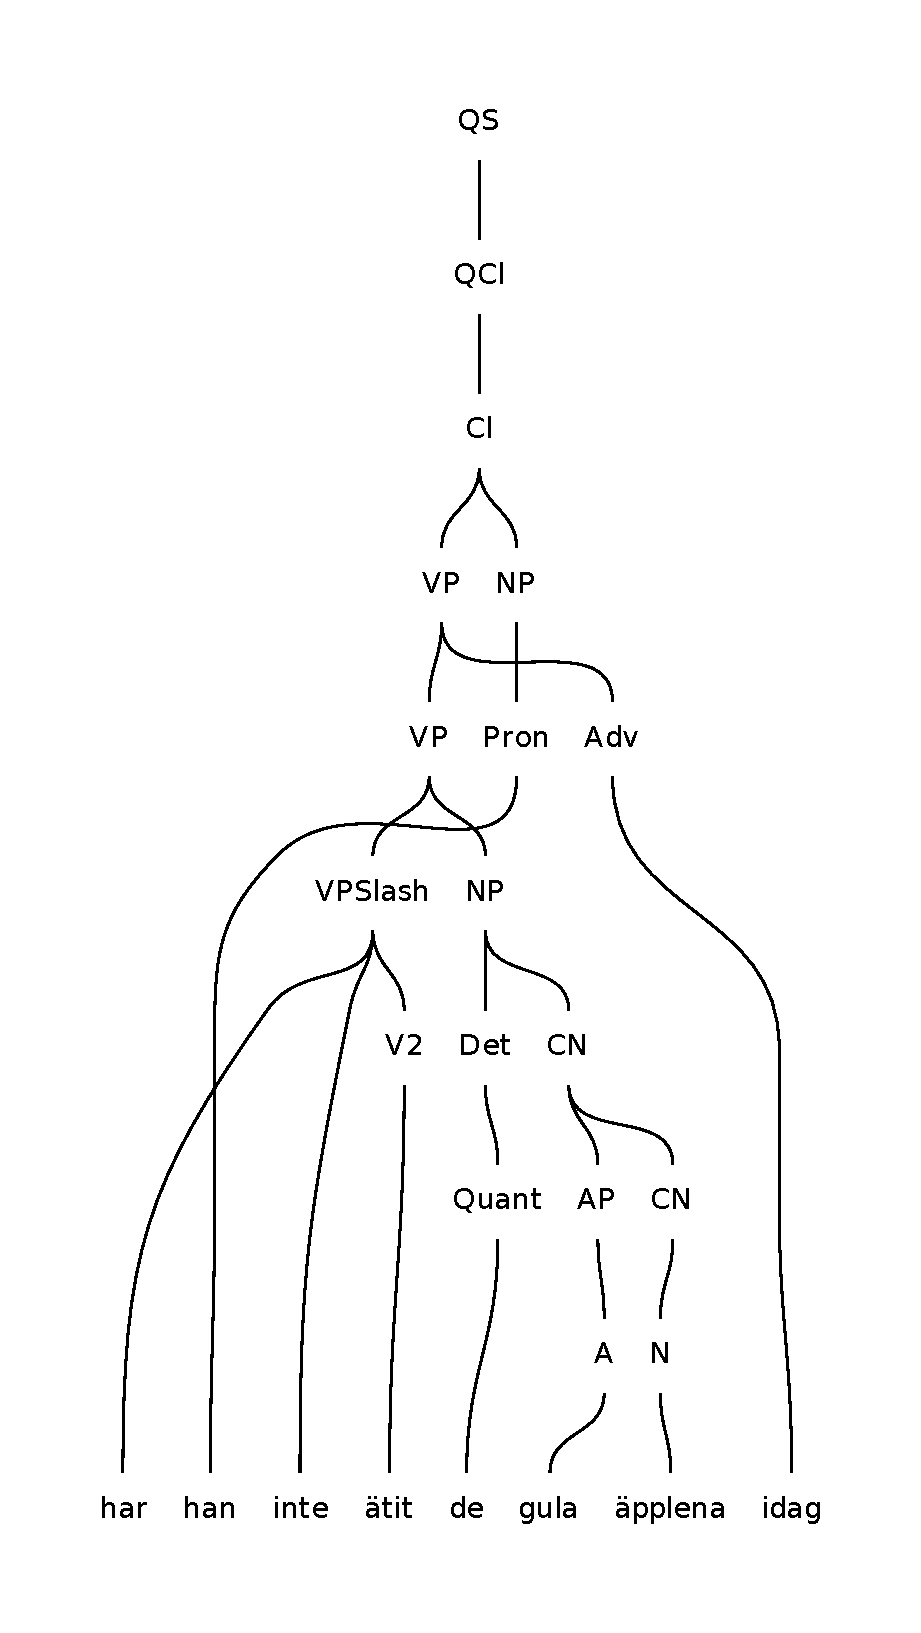
\includegraphics[width=70mm,height=70mm]{apples.pdf}
\caption{Parse tree for ``Han har inte ätit de gula äpplena idag".}%correct
\label{gfSwe:parsetree}
\end{figure}
Even though the verb phrase \emph{``har inte ätit.."} is discontinuous, the whole
phrase is still treated as one constituent in GF. The parts
are connected in the tree, and the subject \emph{``han"} is put between the
finite verb and the rest of the phrase. At the code level, this is implemented
using records.
The linearization rule for questions -- clauses with inverted order -- picks 
the field for the finite verb and appends it to the subject followed by
the negation, infinite part and the complement of the verb phrase: \\
\verb|table { Inv => verb.fin ++ subj ++ verb.neg ++ verb.inf ++ verb.compl ; ... | \\

Relative clauses are also covered: 
\enumsentence{\shortexnt{5}{Hon & ser & pojken & som  &sover}
              {She & sees & the boy & who & sleeps}}
              %{`She sees the sleeping boy'}}

\enumsentence{\shortexnt{6}{Han & ser &katten & han  &tycker & om}
              {He & sees & the cat & he & likes &}}
              %{`She sees the sleeping boy'}}
In addition to the basic resource grammar, additional constructions had been added
to the module \verb|Extra|. The functions given here do not have to be translatable
to all other language, but are meant to cover language specific constructions.
%For example, the \verb|Extra| module included
Among those were functions for topologication, although not all
of them were implemented for Swedish.
%word order, agreement, tempus, adverbs, adjectivs...
%and relatives
%Also info in the Extra module, where more language specific constructions
%can be found.
For example, \verb|FocObj| fronted the object as in sentence \ref{gfSwe:apple}.
\enumsentence{\shortex{6}
{Det & äpplet & vill & jag & inte & ha}
{That & apple & want & I & not &}
{I don't want that apple}}\label{gfSwe:apple}
The module provided functions for preposition stranding:
\enumsentence{\begin{tabular}{ll}
Stranded preposition & cf.\\
Vem måste jag akta mig för? & För vem måste jag akta mig?\\
Who do I need to watch out for? & For whom do I need to wath out?\\
\end{tabular}}

%jag ser dig
%dig ser jag
%dig har jag inte sett
%jag har inte sett dig.
%how the parse tree is generated, the finite verb, the subject, the rest. usw.
%han såg katten han tyckte om
%för vem måste jag akta mig
%vem måste jag akta mig för

%honom ville hon inte tänka på.

Before describing what has been added, will give a short introductions to the
the cats of resource grammar and the sw ipmlementation in particular.

Most important now is NP and VP.
Starting from N, get to CN what is it, what can we do now.
To turn in into a NP need to fix determination, by Det. Dets have .. fixed,
but allow variantion in.. 
What is the difference? Some words on differences for pronouns.
To form \emph{`fågeln'}, the determiner (DetQuant DefArt NumSg) is used.
Example, use vartiants {}.
There are also Quants, which .... 
Once we have a NP, can use Predets. What they are.

For verbs, but also others there is an important distinction for valency.
Either directly to VP if V, or needs to be given arguments. Can then add adverbs.
Maybe talk about ställa.
Particles and prepositions, can't be seen on the trees.
tycka om /tycka om -> om vad tycker du inte. fast bra

%Besides the categories NP,VP,AP there are also the import Det and Quant, Predet.

%What was in the resources
%description of the existing grammar, the types, the possibilities
%VP, NP.
%valency built in (problems with ställa - på, under, vid).
%Determiners, quants, predets, The difference from how pronouns are regarded. 
%Variants, nonexist.
%coverage of standard Swedish.

\subsection{Added}
Summary of what have been added and motivation.

kommer att - for scand, extra tempus, example
example table

%%PASSIV
\subsubsection{Passive}
There are two ways of forming passive verb phrases in Swedish: the 
\textbf{periphrastic passive}, formed by using a modale auxiliary verb \\
\enumsentence{ \shortexnt{6}
{Bilden &blev& tagen& av & rymdsonden & Galileo}
{The picture & was & taken & by & the spacecraft & Galileo}}
\label{gfPass:peri-pass}
or by adding an \emph{s} to
the verb: \\
\enumsentence{\shortex{5}
{Bilden & togs&  av & rymdsonden&  Galileo}
{The picture&  took+\textbf{s}&  by&the  spacecraft& Galileo}
{``The picture was taken by the spacecraft Galileo"}}
\label{gfPass:s-pass}
This second variant, the \textbf{s-passive}, is commonly used in Swedish, some studies
suggest that it is used in more than 80\% of the times \cite{laanemets}.
It is not as common in the other scandinavian languages however, 
and it can not be used in all tenses for all words. The norweigan 
translation of both sentence \ref{gfPass:peri-pass} and sentence  \ref{gfPass:s-pass} is
%The periphrastic passive is preferred, especially in spoken langauge.
\enumsentence{Bildet ble tatt av romsonden Galileo}
The resource grammar for Scandinavian therefore expressed the passive using auxiliary verb. \\
\verb|PassV2 : V2  -> VP | \\
\verb|         ta -> blev tagen| \\
This rules allows two-place verbs to be used in passive by using \emph{bli} (\emph{become}), and thereby
turned into comlpete verb phrases; they no longer need an object.
The s-passive has now been added as the standard case for the Swedish GF
grammar. Periphrastics passive is still allowed, but as an alternative rather
than the default.
The grammar also allows using three-place verbs \verb|V3| , as \emph{give}, to
form passives:
\enumsentence{\shortex{6}
{Betyget & 3 &ges &till &många &elever}
{Grade & 3 & give+\textbf{s}& to & many & students}
{``Grade 3 is given to many students"}}
\label{ex:passV3}
by letting the first object be `removed' and given by the subject. 
A remark can be made about sentences where the second object is put first in the sentence, like 
\enumsentence{Till många elever ges betyget 3}
This is a variant of example \ref{ex:passV3}, \emph{`många elever'} is still the object but put in focus. The grammar
parse this by applying \verb|FocObj|.
%%

%% Clauses
\subsubsection*{Presentering, Impersonal constructions, Topicalisering}
Formal subjects \cite{SAG-19,H&H-309d} is often used in Swedish.
\enumsentence{\shortex{6}
{Det & sitter & en & fågel & på & taket}
{It & sits & a & bird & on & the roof}
{``There is a bird sitting on the roof''}}
\emph{`Det'} has the position of the subject, and the real subject, 
\emph{`en fågel'} the one of an object.
Transitive verbs may not be used like this
\enumsentence{
*Det äter en fågel på taket\\
 ''There is a bird eating on the roof"}

unless their in passive form
\enumsentence{
Det äts en fågel på taket \\
A bird is being eaten on the roof}
A very common example of this is sentences with the verbs \emph{finnas},
\emph{saknas} and \emph{fattas}.
\enumsentence{\shortex{3}
{Det & finns & kaffe}
{It & exist & coffee}
{''There is coffee"}}
\enumsentence{\shortex{3}
{Det & saknas&  kaffe}
{It & misses & coffee}
{''There is no coffee"}}
\enumsentence{\shortex{3}
{Det & fattas & kaffe}
{It & misses & coffee}
{''There is no coffee"}}

A special GF category, \verb|SimpleVP|, was needed for verb phrases of the type
described above.

There are also restrictions on the subject.
\enumsentence{\begin{tabular}{ll}
*Det sitter den fågeln på taket. & *Det sitter fågeln på taket.\\
``There are that bird sitting on the roof'' & ``There are the bird sitting on the roof'' \\
\end{tabular}}
The noun must be in indefinite form, even though some determiners are allowed.
\enumsentence{Det sitter några fåglar på taket\\
              ``There are some birds on the roof''}
\enumsentence{*Det sitter fåglarna på taket\\
``There are the birds on the roof''}
%%Quantifiers like \emph{`denna'} or determiners like \emph{`samtliga'} may
%%not be used, but the determiners \emph{`många'}, \emph{`några'} and the quantifier
%%\emph{`ingen'} work well.
%%Semantic difference, atm we allow any NP. \\
The GF grammar does not make any distinction between indefinite and definite noun
phrases. Therefore this is handled by looking at the determiner. \\
\verb|FormalSub : SimpleVP -> Det -> CN -> Cl ;|\\
The function combines a verb phrase a determiner and a noun phrase in to a clause.
If the determiner requires a noun in determinened form, the clause is put to NONEXIST.
However, this is not an ideal solution. There are other examples of when we
need to know the definitness of the noun phrase, for example when using
the reflexive possessive pronoun `sin' (see section `Reflexive pronouns' below)
or when using some predeterminers (see section `Quantifiers').

%finnas: här får man ha definit: det finns de som inte vill. Samma RelCl som
%jag just la till, de äppplen. (de + relsats)

%'det är kul att..' Näst vanligaste två-ordskombinationen i talad svenska.
%%
%embedded - relative, 'sådan att' not really nice for normal swedish, and no agreement
%between subject 'en katt sådan att det regnar'. Kan säga 'en sån katt som sover, med 'sådan' + Rel
%har lagt till Det äpple + Rel (RelCNNP). *Det äpple är rött. men Det äpple jag äter är rött.
% 


\subsubsection{Quantifiers, determiners and predeterminers}
The GF analyse differs sometimes. Experiments of how to extract
this information from Talbanken by using Saldo as a starting poin.
One of the biggest differences between the GF analysis and the one made in Talbanken
is related to pronouns. While GF only recognizes the personal pronouns, 
`sådan', `fler`, `somliga' etc. are all regarded as pronouns in Talbanken and Saldo.
In the GF analyse they may be quantifiers, determiners or predeterminers. 
All pronouns from Saldo was listed and by searching Talbanken for which tags
they got we could sort out the ones acting either as
determiners, as `sådana' in sentence \ref{ex:QuantDet}, or as adjectives as
`sådan' in sentence \ref{ex:QuantAdj}. 
\enumsentence{Sådana katter vill jag ha}\label{ex:QuantDet}
\vspace{-3mm}
\enumsentence{Han är sådan}\label{ex:QuantAdj}
\vspace{-3mm}
\enumsentence{Sådant är inte bra}\label{ex:QuantDet2}
Since all determiners can be used alone as noun phrases, sentence
\ref{ex:QuantDet2} is also accepted.
%what is the difference really???
%The techniques of searching Talbanken can be used
%for this purpose as well. 
%combining the information in Saldo and Talbanken
%pronouns/Quant. Many, created categories for 'sådan', and 'fler'. Not many in each,
%has to decide, one category for each?

\subsubsection{Other small things}

\textbf{Genitive} -problem 1 cannot be alone (fixed) 2 some words have id. (no) gen form (fixed)
           fixing this include restructuring all???
\textbf{Det-utr}. not effect for the some Dets, like 'sådan', no difference between utrum and neutrum.
 Can vary in number, since is a NP. Do not want to cut connection to abstract but changing them,
 so added one more. Leads to ambiguities in some cases, but considering that we would want to use
 this for translation, neutr and utr may differ in the other language.

\textbf{finitness}
 'de flesta de gula hästarna'

\textbf{advs}
-- or is this really just AdVs? 
to change position of adv:
normal: after verb 'han äpplet redan'
now want: 'äter redan äpplet'
          'har redan ätit äpplet' 
          'har ätit redan äpplet' :( which doesn't work either :)

\textbf{bara}
but have other words like 'bara' which can be put in other positions.
  but needs to restruct whole of VP, since no field is befor fin.
  Can also act before the noun or as AdV. Examples.
\verb|s SPres Simul Neg Main : han bara sover inte alltid|
  have added a field in VP, a0, show table.
  makes some weird constructions when using modal verbs, 
  \verb|s SPres Anter Pos Main : han bara har alltid sovit|
  but rather than changing to 'han har bara sovit', we keep it. Is a possible
  tolkning and the other case is covered by using it as an AdV, we don't want
  ambiguities.

\textbf{antalet}
Also needed categories for 'pronouns' wich can act in different ways.
and 'antal','sorter' - need indetermined, antal plural, sorter either.
Should be able to modify by a godtyckligt antal adjective, and they must be determined.
'(ett stort antal) människor' and not 'ett stort (antal människor)'
Don't want them as a NPs or CNs since we don't want other Ns to be used this way
'en flicka kaffe', this is then Appos? (Or do we?). Should also not be utsatta for what other
NPs or CN can be. Dessutom, we want to make use of the comp-fiel. 'mamma till', but is this really
the same??

\textbf{VP}
The VP require many changes PPart, bara.
About PPart, but do we need it with new Saldo? 'de är stuckna' , 'den nyligen funna'
for the last one, we need VPSlash to allow adverb.

\textbf{SuperlA}

\subsubsection*{Reflexive pronouns}
%varandra and sin/sitt/sig.
Both sig and sin
Not subject, but NP.
Want the following:
\enumsentence{Han såg sina barns skor.}
\enumsentence{Sina vantar hade han glömt på tåget.}
but not
\enumsentence{*Sina vantar var kvar på tåget.}
\enumsentence{Han ger sina pengar till sina syskon.}
\enumsentence{*Jag ger sina pengar till sina syskon.}
\enumsentence{Han är längre än sin kompis.}
\enumsentence{Hon tyckte om alla sina elever.}
\enumsentence{Han såg sin hund och sitt hus}
\label{ex:refGen}
\enumsentence{Han är längre än sin kompis}
\label{ex:ReflAP}
% hon ber sin katt gå - sin subject in clause.

Suggest a connection between the subject and the object.
Could be combined with 'sig', a ReflNP without another noun.
-- man ser sig!!
Make a distinction between objects and subjects?
do not want to copy all rules for another category. Would like depent types!
work pretty well by letting all NP depend on the subject in the phrase.
The current version is nice and works for recursive genitivs!
Extra info, but maybe this is just the case about NPs.
Discuss how other solutions, NPR and Predet : Predet -> CN -> NPR ;
*Slash* : VPSlash -> NPR -> VP ;
Keep number of fields down, but introduces another category, and one more
label to the parse tree, is it interesting? How to combine it with genitive 
without making it ambiguous (Han såg barnens hund).
What if we add alot of other rules that uses NP, will they all need to be
duplicated then?

'han såg sin mammas bil', they same could be applied to
APs for example \ref{ex:ReflAP} or Adv for
\enumsentence{Han leker oftare än sin kompis}
 (ComparAdvAdj)
Atm you can't focus this kind of object, then a ClSlash need info about the
subject. FunRP also tricky (and what does it mean, we can say
Han såg sin katt i vilken musen låg), in this case RP needs to give more information.
Kort sagt, the information about the subject must be spread
in different parts of the sentence. 
Could also decide to always produc 'sin' -> jag såg sin bil
to avoid the dependence, but not nice. Or keep a flag in NP saying if it is
in third person, and add nonexist for others. But this way we can also get rid
of ReflVP and the possessive prons \verb|PossPron| should only be used for somebody else:
'jag såg din bil'.
Unfortunaly, have to change ReflVP, this only allows this in object for VPSlash, not FocObj,
not 'alla sina', usw. Want it to handle conjuction as in example \ref{ex:refGen}
etc.
varandra, works the same but has no case for Sg.
Johan vill att jag rakar sig* -> honom  
%%

In general, many categories need more parameters and fields, tex Quant can be used as NP
and therefor needs to depend on Case, de -> dem.

here or in robust: SupCl, det as VP or VV or S for S (remember Foc)
\subsubsection*{Relative clauses}
The resource grammar already provided a number of ways to express relative and embedded clauses, such as
\enumsentence{Frågan är vilken färg den har\\
                   Pojken, som är blyg, tystnar\\
                   Han såg kunden som tyckte om sallad\\
                   Jag tänkte på huset i vilket hon bodde} % better example!!

Kanske mindre om detta, skriv om vad jag nu la till.
om 'de äpplen', which are also used in 'finnas'
Since those constructions are inspired by other languages, some of them may sound quite
non-natural in Swedish, such as the \verb|RelS|. This combines a sentence \emph{`Hon sover'}
and a relative sentence \emph{`som/vilket är bra'} which wrongly expressed 
\emph{`She sleeps, which is good'} as
\emph{`Hon sover som är bra'}. The error comes from the fact that \emph{`som'} is
embedded in the relative clause. To fix this, an extra parameter was needed to tell whether
\emph{`som'} or \emph{`vilket'} should be used. \\
Another complication stems from \verb|RelCl| which express the english \emph{`such that'}.
The Swedish version \emph{`sådan att'} sounds stelbent, when used outside of logic books.
\enumsentence{Jag vill ha en katt sådan att den inte fäller.} 
An more natural sounding alternative would be
\enumsentence{Jag vill ha en sådan katt som inte fäller.}
and hopefully this will be implemented soon, otherwise: why is it hard and how we can say
'en katt sådan att det regnar'. It is relative but has on empty field, still congruation is
needed.
du är här, vilket jag vet.
i de äpplen/det äpple du äter bor en mask/ som du ser.\\


\subsection{Testing}
Hard do test, can't verify. Regression testing. Talbanken is still too hard.
While developing: regression, 150 sentences to start with. Made longer, both good and bad,
to see how many ways things can be parsed.
Test how many parse trees that are generated.
Look at tables for a VP tex.
Some results.

% One part about the grammar. The state of the original grammar, what was covered and not. 
% What parts that I have been working on and why, 
% what constructions I wanted to add, examples of sentences that should work
% and of sentences that shouldn't be covered. How to separate Swedish from
% Scandinavian, bigger reconstructions in the grammar. 
% sammanhängande explanation of the swedish grammar, choices I have made, why
% regression testing

\section{Mapping}
\label{sec:Mapping}
Talbanken contains much valuable information about phrase structures and word 
usage. One part of this project has focused on extracting this information
and to translate it to GF notaiton. We have constructed a mapping, which 
automatically transforms trees in Talbanken format to GF abstract syntax trees.
Figure \ref{fig:translationtrees} shows an exapmle of a visualized tree
from Talbanken05 and the result of translating it to GF.
Both the POS tags as well as the syntactic information are needed for the translation.

\begin{figure}[h]
\centering
\subfloat[Talbanken tree]{\label{pic:tbtree}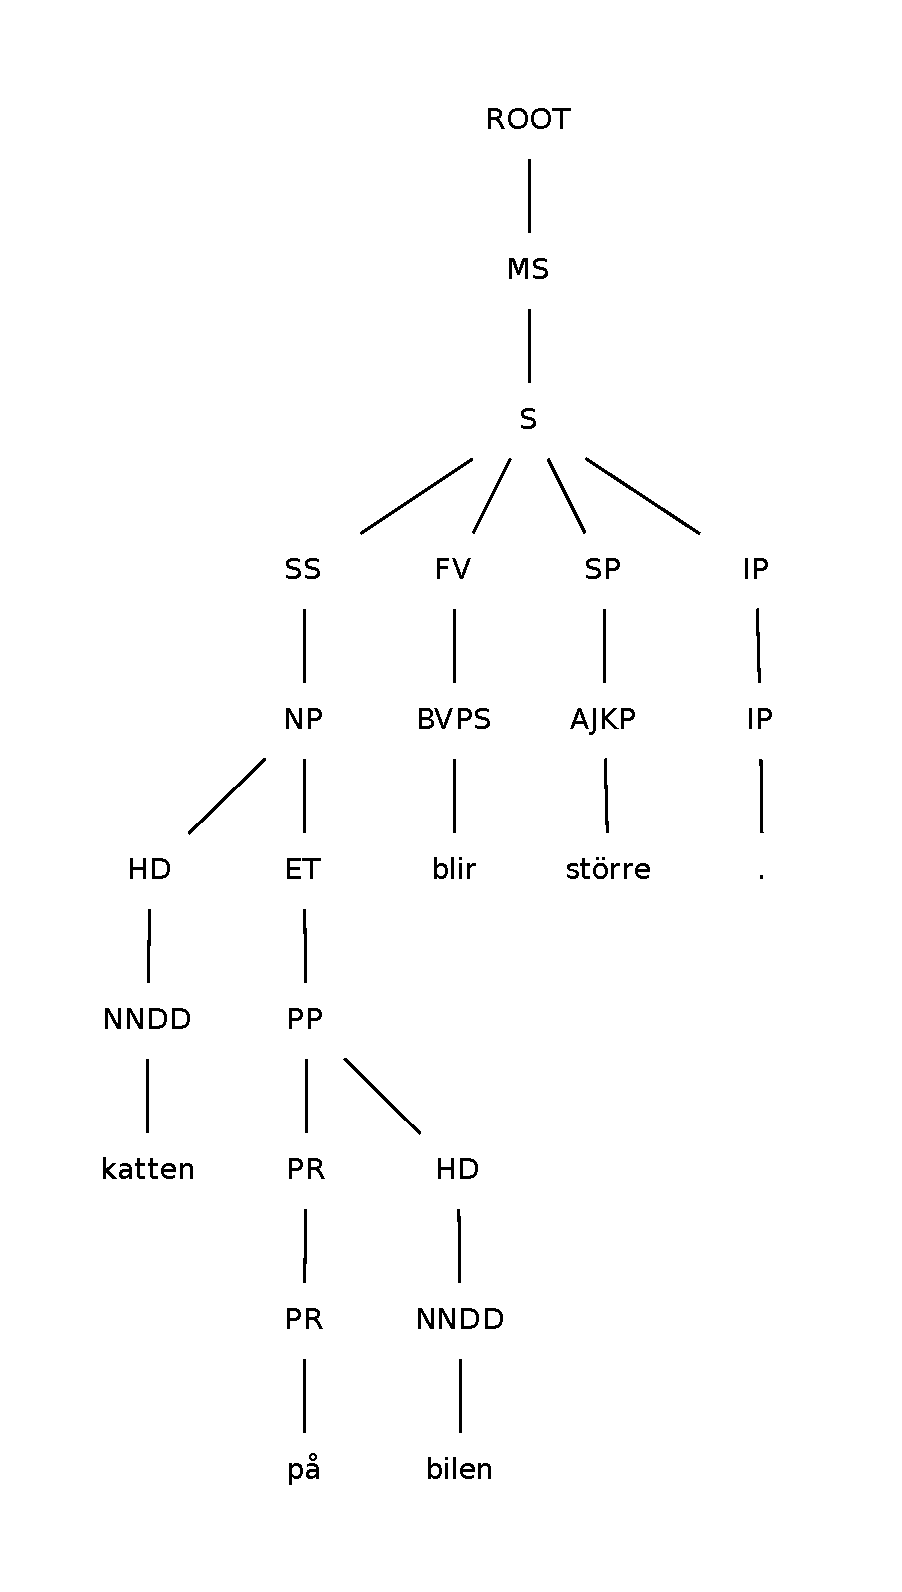
\includegraphics[width=60mm]{Talbankentree.pdf}}
\subfloat[GF abstract tree]{\label{pic:gftree}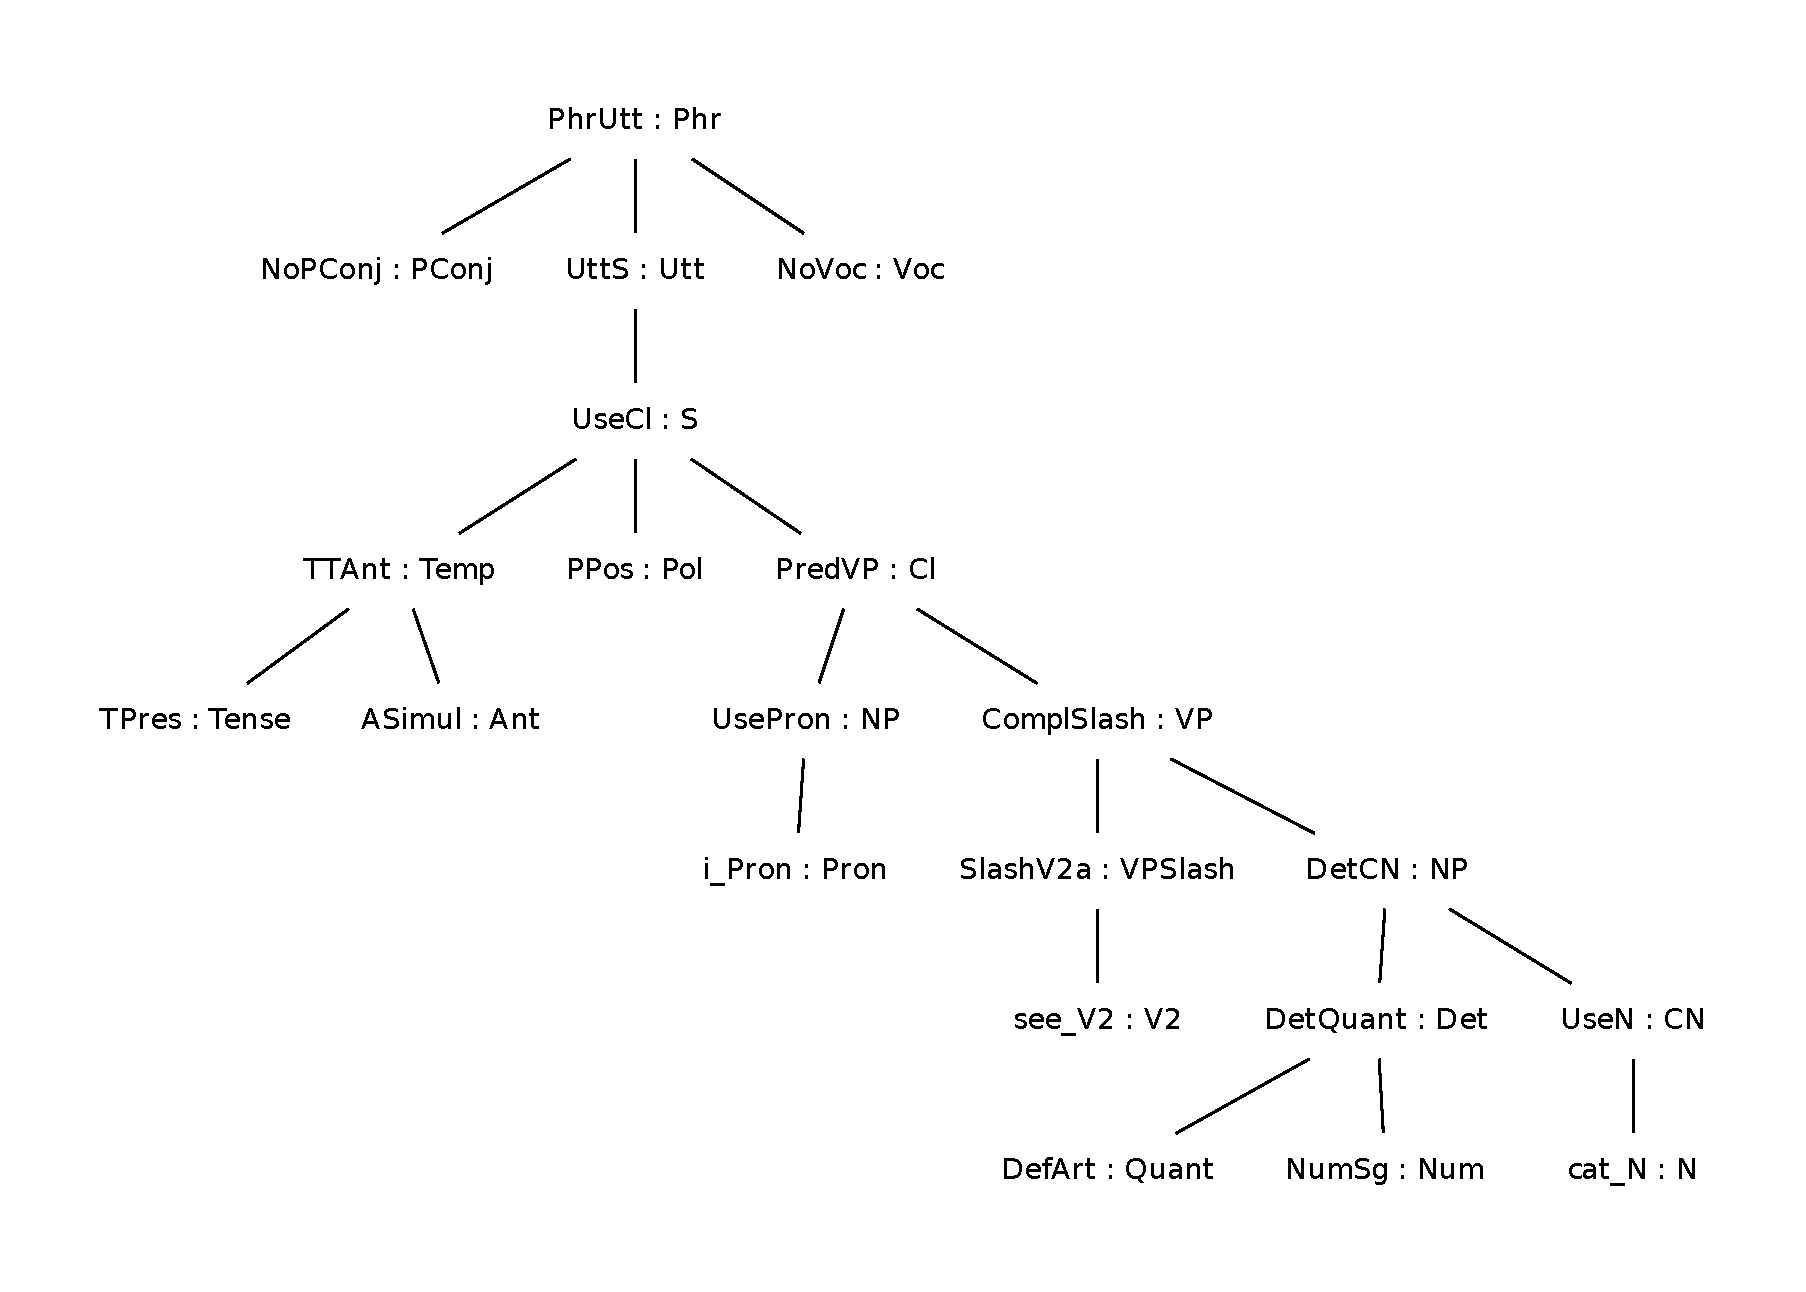
\includegraphics[width=60mm]{gfTree.pdf}}
\caption{Trees for the sentence ``Katten på bilen blir större".}
\label{fig:translationtrees}
\end{figure}

The mapping connects GF with another annotations and gives us means to evaluate
our parser. By both parsing a talbanken sentence and transforming its annotaded tree, we can
easily inspect if the results are equal.
The mapping also makes it clear which grammatical constructions that are still missing
from the GF grammar and shows how the GF analysis differs from the one made
in Talbanken.
If there are words missing from our dictionary, the rich
pos-tags may help us to automatically find the correct declination and add it to the
lexicon. Further, our parser will need probabilities, see section
\ref{sec:future}, of how often a function is used.\\
%missing words. Lexical aquisation, probabilities, see section .
%The mapping gives information about which form a word is
%currently used in and this may be used by the lexical extraction
%tools. % Those can be enhanced if they are given more data. 
%The translated trees enable us to extract those probabilities. %The mapping gives us a source for this.
%Furthermore, the translation makes it easy to identify grammatical constructions
%missing from the GF grammar Another important use of the mapping is evaluation of the parser, which can be
%accomplished by comparing the parse trees and the trees from the transformer.

A program for translating trees to GF syntax has been done before (Angelov,).
It translated trees from the English Penn Treebank. By starting this progam, we now have
a translation that works for the quite differently annotated Talbanken. The differences between
Swedish and English syntax also meant that many rules had to be changed.\\

The mapping works for Talbanken05 in Tiger XML-format. There are three kinds of
tags: categories, edge labels and pos tags. 
The categories give syntactic information such as \verb|S|,\verb|NP| and \verb|VP|.
The edge labels give similair information with tags as \verb|SS| for subject, 
\verb|OO| for object. There are more than 300 different pos tags. The high
number is due to the detailedness, for example there are almost 50 tags for
nouns, excluding proper names. The tags show definitiness, case, whether the
word is a compound. Some words also have their own tags.\\

\begin{tabular}{lll}
\textbf{Tag} & \textbf{Example} & \textbf{Explanation} \\
\hline
\textbf{SV} & ska & The verb \emph{shall}\\
\textbf{WVIV} & vilja & The verb \emph{want} in infinitive\\
\textbf{KVSP} & kommit att & The verb \emph{will} in supine\\
\textbf{GVPT  PA} & gjordes & The verb \emph{do, make}, present, passive \\
\textbf{NNDDHSGG} & familjemedlemmarnas & Noun, definite, compound (person), genitive \\
\textbf{PU} & *, 1), a) & List item  ...\\
\end{tabular}\\

%Pos continues
%to either new tree or a word. Example S -> PP -> (Hd -> Id , Hd -> Id). Show
%corresponding GF tree.

The translation works sectionwise, ie, if it finds a tree of category \verb|S|,
it will start to look for a subject \verb|SS| and a finite verb \verb|FV|. If it
can find those, they can be combine with the GF function \verb|PredVP|.
At the lowest level in the tree we look up the word in the GF lexicon.
It figure \ref{pic:tbtree}, the verb is followed by an adjective as a present
participle, \verb|SP|. GF admits \emph{bli} to have type \verb|VA|, a verb
with an adjective as complement, and the translator can apply the gf function
\verb|ComplVA| to combine the verb with its object. \\
It is not often the case that we can first find the subject, then the verb and 
finally the objects. Often the order is Verb-Subject-Object or Object-Subject-Verb. \\
During the mapping process, the translator also needs to find out whether the sentence is
negated and what tempus is used. If it finds two trees of type, say, \verb|VP| but does not
have any rules for combining them, the \textit{meta function} \emph{'?'} will be used. 
Figure xx shows an exapmle of this.\\

%How we try to build up a 'abstract syntax tree', a S with a NP VP for example. 
%Continue with dividing VP into Verb Objs. More possible word orders (or at
%least more commonly used). 'katten åt sin mat fort' 'åt katten sin mat fort' 'sin mat åt katten fort'
% If can't find, add a '?', a meta.
%This is also what happens when the translator finds a combination it doesn't know about.
%Example of tree with meta.

%Description of most important tags from Talbanken, their translation? appendix?
The structural differences between GF and Talbanken cause some translation problems.
On example is that Talbanken has no valencey information but for GF this is the key when
constructing for example verb phrases. The grammar bestämmer that a transitive \verb|V2|
needs by two objects. The distinction is not always clear in Swedish where 
most transitive verbs can also be used as intransitive. Both sentences in
example \ref{ex:mappTransitive}.
\enumsentence{Han sitter och läser.\\ Han sitter och läser en bok.} \label{ex:mappTransitive}
See section \ref{sec:futureValency} for a longer discussion about this.
For this reason, the mapping will allow words to be used in other ways than their
GF valencies prescribes.

Another problem can be instantiated by sentence \ref{ex:mappMan}, containing the generic pronoun \emph{man}.
\enumsentence{Man uppskattar dem.\\
        \emph{They are appreciated}}\label{ex:mappMan} %  (s216).
In talbanken, \emph{man} is simply a personal pronoun, 
in GF it causes the whole clause to get the form \verb|GenericCl|, which has no
subject visible in the abstract tree. See figure \ref{fig:mappMan}.
\begin{figure}[h]
\centering
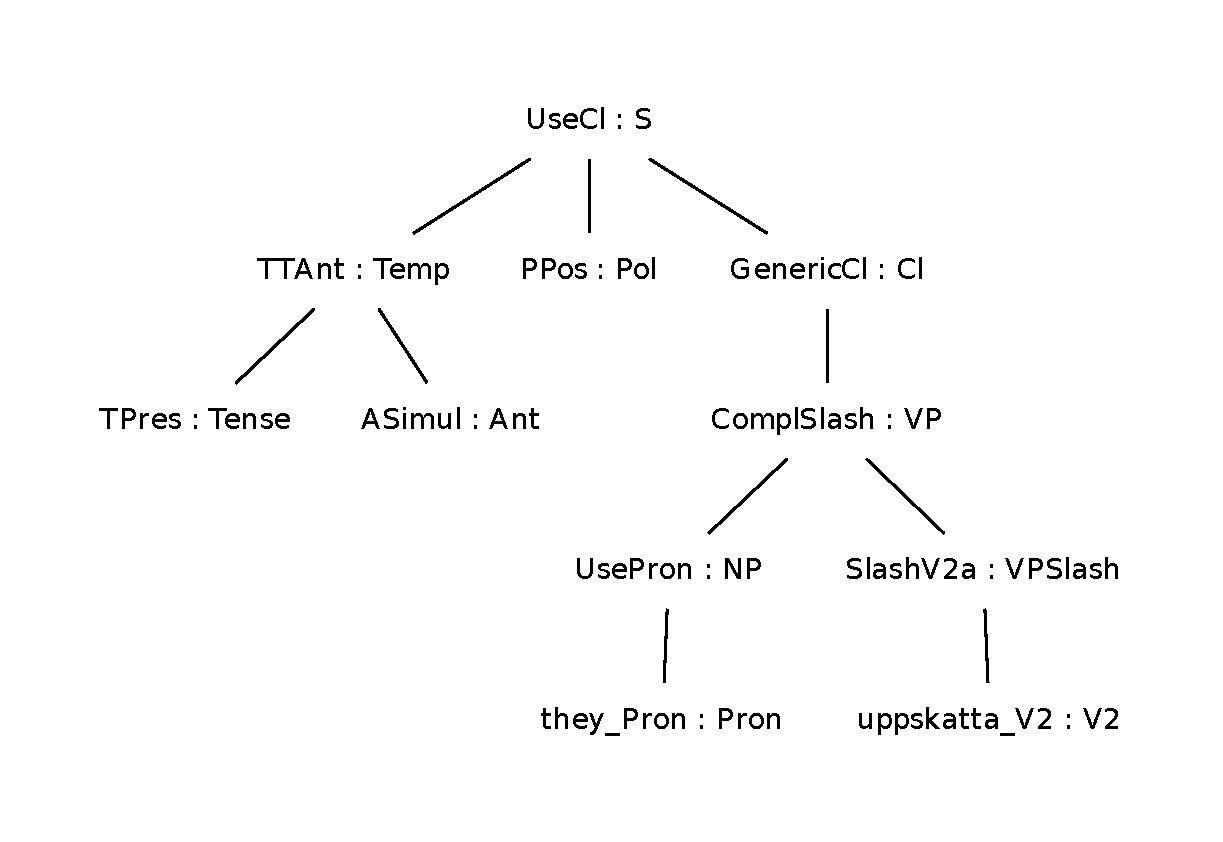
\includegraphics[width=80mm]{man.pdf}
\caption{Abstract tree for ``Man uppskattar dem".}
\label{fig:mappMan}
\end{figure}
In this case, it is not possible to simply glue the subject to the verb with \verb|PredVP|.
%Therefore, the translator must change the type of the 
%sentence when inside the SS.

%förklara bättre eller ta bort??
A similair issue arises form the use of verb particles. If a verb with a particle is considered
as one klump in GF, which means that the particle has no effect on the abstract tree. Its presence
is announced by the verb itself. The lexicon may contain a verb both with and without a particle,
for example \emph{tänka} (think) and \emph{tänka till} (consider?).
\begin{verbatim}
taenka_V  : V ;
taenka_till_V : V ;
\end{verbatim}
When the translator looks up a the form \emph{tänka}, both of the two verbs
will be among the results. The first option will be selected, and if the
particle isn't directly attatched to the verb
%There is, at this point, no easy way of knowing which one of them wants a particle and the
the transformation might confuse the two words. This is also the case when translating
all sorts of idioms that GF considers to be just one bit.\\

%Difficulties in looking up 'idioms' like this
%in the gf lexicon. Therefore the translator might get confused.
%Sentences are also differntly deep. Example of a conjuncted sentence.

On of the reasons why \textit{metas} are put in the output, is the 
use of tags like \\
\begin{figure}[h]
\begin{tabular}{ll}
\textbf{NAC} & Not a constituent\\
\textbf{XP} & Other (non-coordinated) phrase\\
\textbf{DB} & Doubled function\\
\textbf{PU} & List item\\
\textbf{XX} & Unclassifiable part-of-speech\\
\end{tabular}\label{fig:mapBadtag}
\end{figure}

They occure quite frequently in the treebank and are always translated
to \emph{?}.
%How we cannot cover all cases. 

\subsection{Results and evalutaion}
The flat version of Talbanken05 was used for developping the mapping, but
the program works for both versions.
The deeper contains six more tags, but they are not always useful for our       
purpose. Figure \ref{fig:mappDeepFlat} shows the difference for a conjunction.
% show piece of s5 here!
\begin{figure}[h]
\centering
\subfloat[Deep]{\label{pic:mappDeep}
\includegraphics[width=20mm]{nofile.png}}
\subfloat[Flat]{\label{pic:mappFlat}
\includegraphics[width=20mm]{nofile.png}}
\caption{...}
\label{fig:mappDeepFlat}
\end{figure}

Some more information about VP are given by the tag \verb|VG| (\emph{verb group}),
which can group an infinite verb and an object abverbial together into a \verb|VP|.
This information can however be extracted from the flat version, and the results
get slightly better when using the flat version. \\


%At least one rule  and also most of the
The development was mostly example-driven, and at least one rule for each
Talbanken-tag has been implemented.
Shorter sentences have been prioritized in order to get a coverage of the most
fudamental constructions. Further,  
regression testing was used during the development. % in order to  very easy to destroy what was working before. 

When evaluating the mapping, the results depend a lot on the restrictions on the
input. 
The focus has been on shorter sentences, with no idioms or conjunction. We are
not interested in sentences made up by list, since they are meant for making
a nice graphic look in folders etc.\\


If we
assure that the lexicon know the correct word class for all lemmas involved, we
can restore more than 85\% of the nodes in the original tree.
If we lift all the restrictions excluding the \verb|PU|, we get
%When tested the 100 first sentences from Talbanken, we get
65\% coverage.
If we test randomly collected sentences that does not contain and any of the tags listed
in figure \ref{fig:mapBadtag} 72\% can be restored. \\

\begin{tabular}{ll}
No list items & 65\%\\
No special tags or punctiation & 72\%\\
Short sentences with known words & 85\%\\
\end{tabular}

%If we don't take the verb valency into account, allow all verbs to have Gf category V,
%we get a slightly better result,
%from 62.5\% to 65.4\%.  (see EvalText). The complemnt of the verbs should tell which category
%they are anyway.
%Evaluation. -> Works for both flat and deep, but with sligthly better results for the flat one.

% hard examples like
% ger sig till henne -> ReflSlash ge henne in gf
% questions with objects that should be moved
% vilken katt såg du
%This part explains
%the tags in Talbanken and gives examples of how they are translated,
%examples of what can be parsed and what cannot.
%about how to make the code work for swedish, differences
%regression testing


\chapter{Summary}
\section{Results and discussion}
Results from mapping, can probably be improved, bit by bit, depends much on words.
Valencys would therefor help.  
Saldo, made a big difference to renew the lexicon. Tested what was missing now from talbanken,
results. Mostly compound nouns, which we can't expect in the dictionary.
Is too slow, can't be used for parsing right away

Grammar - hard to evaluate automatically, but Elibet is an expert who has been involved
in the process to verify the solutions. Testing trees against talbanken.
The big lexicon makes it very slow, eats all memory

Discussion of the results and methods, why are the results good, why are they not better.
What other methods could have been used? What did we/I expect and what happend?


\section{Future Work}
\label{sec:future}
What is still left to do? Description and direction of future work:
Handling unknown words and , handling unknown grammar, 
how to make the parser robust, elipses and long sentences, names and numbers.
What is still needed in the grammar, how important that is. 
\subsection{Lexicon/Parallell parsing}
Speed up.
\subsection{Valency}
\label{sec:futureValency}
how to get valency information 'sitter och läser',
is this doable for swedish?
description of extracting this from talbanken/korp
or handling it by the robust parser or the grammar itself (leaveout obj?).
make the parser faster by using smaller lexicon.
Lexicon tool on the fly.
\subsection{Probabilites}
\label{sec:futureProbabilities}
Getting and using probabilities, to disambiguate.
process list from saldo.
Use multiligual treebank?
stop ambiguities by fixing so that Gen of a quant isn't a quant, or better, that all fields
have a genitive field.
More fields in the grammar? Or leave it all to the robust parser


\section{Conclusion}
There is obviously a lot do still, will never get finish with NPL.
Grammar may need even bigger changes, to allow enough but not too much.
Different from writing a grammar for generation.
Results from mapping shows that the translation is doable, but becomes harder
since talbanken don't have formal rules.
The saldo shows how easy to make use of utomstående resources, promising if
we want to extract other information. 
Hard, but not finished! 


\end{document}
